\subsubsection{Countering the Cyber Attack Kill Chain}
\label{sec:killchain}
\glsresetall
The main concepts of the cyber attack kill-chain are introduced in chapter \ref{sec:killchain-work}. The three most widely acknowledged and used cyber attack kill-chain approaches are the Lockheed Martin ``Cyber Kill Chain'' (Fig.\ref{fig:ckchain}) \cite{LockheedMartin2018}, Mandiant/FireEye ``Attack Lifecycle'' (Fig.\ref{fig:alcycle}) \cite{FireEye2018}, Microsoft ``Attack Kill Chain'' (Fig.\ref{fig:akchain}) \cite{Microsoft2018}, SANS ``The Industrial Control System Cyber Kill Chain'' \cite{SANS-ICS}, and MITRE ``ATT\&CK'' \cite{MITRE-ATTACK}. When compared, the differences between the proposed methodologies are different. Lockheed Martin puts the most effort in identifying and stopping the attacks in their early stages but does not focus too much on the adversary performed activities internally. Mandiant/FireEye, on the other hand try to grasp both initial and internal attack stages in a very broad strokes, not being too granular on every specific stage. However, Microsoft proposed approach elaborates very deeply on the malicious activities performed within the network, but leaving the initial attack stages not deeply covered. All of these methods have their strengths and weaknesses, but when rationally combined should provide the most comprehensive approach bringing out the most important stages of the attack. From a different angle, MITRE ATT\&CK maps adversarial \gls{tttp} to the various stages of the attack preparation\footnote{MITRE PRE-ATT\&CK Matrix. \url{https://attack.mitre.org/matrices/pre/}. Accessed: 27/10/2018} and execution \footnote{MITRE ATT\&CK Enterprise Matrix. \url{https://attack.mitre.org/matrices/enterprise/}. Accessed: 27/10/2018}. Also, SANS proposed kill-chain complies with the main attack stages, as described by other approaches, but adds extra nuances related to learning and targeting the industrial control systems and processes.

\begin{figure}[!htb]
    \centering
    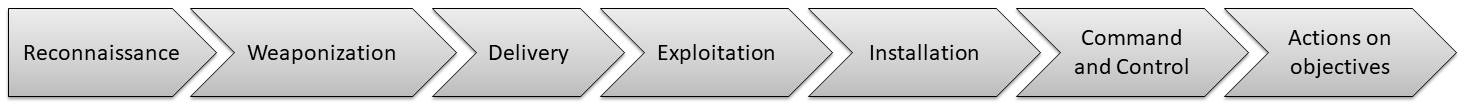
\includegraphics[width=1.0\textwidth]{./img/cyber-kill-chain.jpg}
    \caption{Lockheed Martin Cyber Kill Chain \cite{LockheedMartin2018}}
    \label{fig:ckchain}
\end{figure}

\begin{table}[!tb]
\centering
\resizebox{\textwidth}{!}{%
\begin{tabular}{|p{2cm}|p{2cm}|p{2cm}|l|c|c|c|}
\hline
\textbf{\begin{tabular}[c]{@{}l@{}}Cyber\\ Kill Chain\end{tabular}} & \textbf{\begin{tabular}[c]{@{}l@{}}Attack\\ Lifecycle\end{tabular}} & \textbf{\begin{tabular}[c]{@{}l@{}}Attack\\ Kill Chain\end{tabular}} & \textbf{\begin{tabular}[c]{@{}l@{}}Cyber Attack\\ Kill Chain\end{tabular}}                   & \textbf{Pub.I}    & \textbf{Pub.II}   & \textbf{Pub.III}  \\ \hline
Reconnai-ssance                                                     & Reconnai-ssance                                                     &  Reconnai-ssance                                                     & \begin{tabular}[c]{@{}l@{}}Reconnai-\\ssance\end{tabular}                                    & S                 &                   &                   \\ \hline
Weaponization                                                       & Initial compromise                                                  & \begin{tabular}[c]{@{}l@{}}Initial\\compromise\end{tabular}          & \multirow{4}{*}{\begin{tabular}[c]{@{}l@{}}Initial\\ compromise\\ and foothold\end{tabular}} & \multirow{4}{*}{S}& \multirow{4}{*}{X}& \multirow{4}{*}{} \\ \cline{1-3}
Delivery                                                            & Foothold                                                            &                                                                      &                                                                                              &                   &                   &                   \\ \cline{1-3}
Exploitation                                                        & Escalate privileges                                                 &                                                                      &                                                                                              &                   &                   &                   \\ \cline{1-3}
Installation                                                        &                                                                     &                                                                      &                                                                                              &                   &                   &                   \\ \hline
\begin{tabular}[c]{@{}l@{}}Command and\\ control\end{tabular}       &                                                                     &                                                                      & \begin{tabular}[c]{@{}l@{}}Command\\ and control\end{tabular}                                & X                 &                   &                   \\ \hline
                                                                    & \begin{tabular}[c]{@{}l@{}}Internal\\ reconnai-\\ssance\end{tabular}& \begin{tabular}[c]{@{}l@{}}Internal\\ reconnai-\\ssance\end{tabular} & \begin{tabular}[c]{@{}l@{}}Internal\\ reconnai-\\ssance\end{tabular}                         & S                 &                   &                   \\ \hline
                                                                    & \begin{tabular}[c]{@{}l@{}}Lateral\\ movement\end{tabular}          &                                                                      & \begin{tabular}[c]{@{}l@{}}Lateral\\ movement\end{tabular}                                   & X                 &                   &                   \\ \hline
                                                                    &                                                                     & \begin{tabular}[c]{@{}l@{}}Local privilege\\ escalation\end{tabular} & \multirow{4}{*}{\begin{tabular}[c]{@{}l@{}}Privilege\\ escalation\end{tabular}}              & \multirow{4}{*}{} & \multirow{4}{*}{X}& \multirow{4}{*}{S}\\ \cline{1-3}
                                                                    &                                                                     & \begin{tabular}[c]{@{}l@{}}Compromise\\ credentials\end{tabular}     &                                                                                              &                   &                   &                   \\ \cline{1-3}
                                                                    &                                                                     & Admin hunting                                                        &                                                                                              &                   &                   &                   \\ \cline{1-3}
                                                                    &                                                                     & \begin{tabular}[c]{@{}l@{}}Remote code\\ execution\end{tabular}      &                                                                                              &                   &                   &                   \\ \hline
                                                                    & Persistence                                                         & \begin{tabular}[c]{@{}l@{}}Domain\\ dominance\end{tabular}           & Persistence                                                                                  &                   & S                 &                   \\ \hline
                                                                    &                                                                     & \begin{tabular}[c]{@{}l@{}}Remote code\\ execution\end{tabular}      & \multirow{3}{*}{\begin{tabular}[c]{@{}l@{}}Asset\\ reconnai-\\ssance\end{tabular}}           & \multirow{3}{*}{S}& \multirow{3}{*}{} & \multirow{3}{*}{} \\ \cline{1-3}
                                                                    &                                                                     & \begin{tabular}[c]{@{}l@{}}Asset\\ reconnai-\\ssance\end{tabular}    &                                                                                              &                   &                   &                   \\ \cline{1-3}
                                                                    &                                                                     & \begin{tabular}[c]{@{}l@{}}Local privilege\\ escalation\end{tabular} &                                                                                              &                   &                   &                   \\ \hline
\begin{tabular}[c]{@{}l@{}}Actions on\\ objectives\end{tabular}     & \begin{tabular}[c]{@{}l@{}}Complete\\ mission\end{tabular}          & Asset access                                                         & \multirow{2}{*}{\begin{tabular}[c]{@{}l@{}}Objective\\ completion\\   \end{tabular}}  & \multirow{2}{*}{S}& \multirow{2}{*}{X}& \multirow{2}{*}{X}\\ \cline{1-3}
                                                                    &                                                                     & Exfiltration                                                         &                                                                                              &                   &                   &                   \\ \hline
\end{tabular}%
}
\caption{Cyber attack kill-chain grouping and mapping to countering techniques in publications}
\label{tab:achain}
\end{table}

\begin{figure}[!htb]
    \centering
    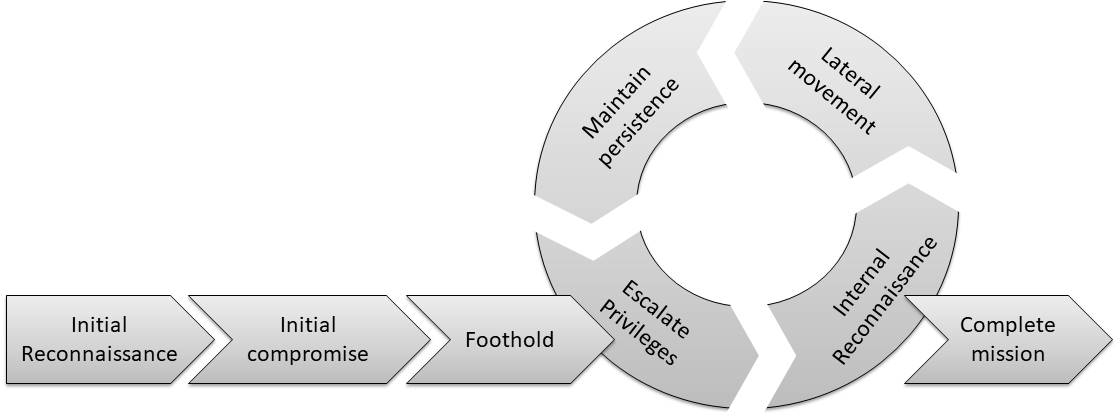
\includegraphics[width=0.7\textwidth]{./img/attack-lifecycle.jpg}
    \caption{Mandiant/FireEye Attack Lifecycle \cite{FireEye2018}}
    \label{fig:alcycle}
\end{figure}

By design the cyber attack kill-chain is developed from the defensive perspective to eliminate the adversarial threat and cyber attack at every stage of its execution. When considering the kill-chain from the attacker's perspective it is critical to be able to counter the kill-chain by applying novel \gls{tttp} to successfully execute every attack stage without being detected and disrupted. Therefore, cyber red team engaged in computer network operations have to employ adequate \gls{tttp} to raise the level of success.
The table \ref{tab:achain} on page \pageref{tab:achain} attempts to represent the stages of every individual approach, and groups them to create the cyber attack kill-chain with the most important stages of the attack, to give enough detail to the initial attack, internal lateral movement, and asset reconnaissance stages. In the table, the \textit{`X'} denotes, that a particular technique is directly applicable for countering a particular stage of the cyber attack kill-chain, and \textit{`S'} identifies, that this method can be used to support countering that particular stage in combination with other applicable approaches and tools.
The cyber attack kill-chain stages are mapped against the methods and techniques presented in the publications, which are applicable to countering or mitigating the effects of every cyber  attack kill-chain stage. This allows the \gls{crt} to adapt and assess their \gls{ttp} applicability to allow the \gls{cno} execution with a higher success rate.

\begin{figure}[!htb]
    \centering
    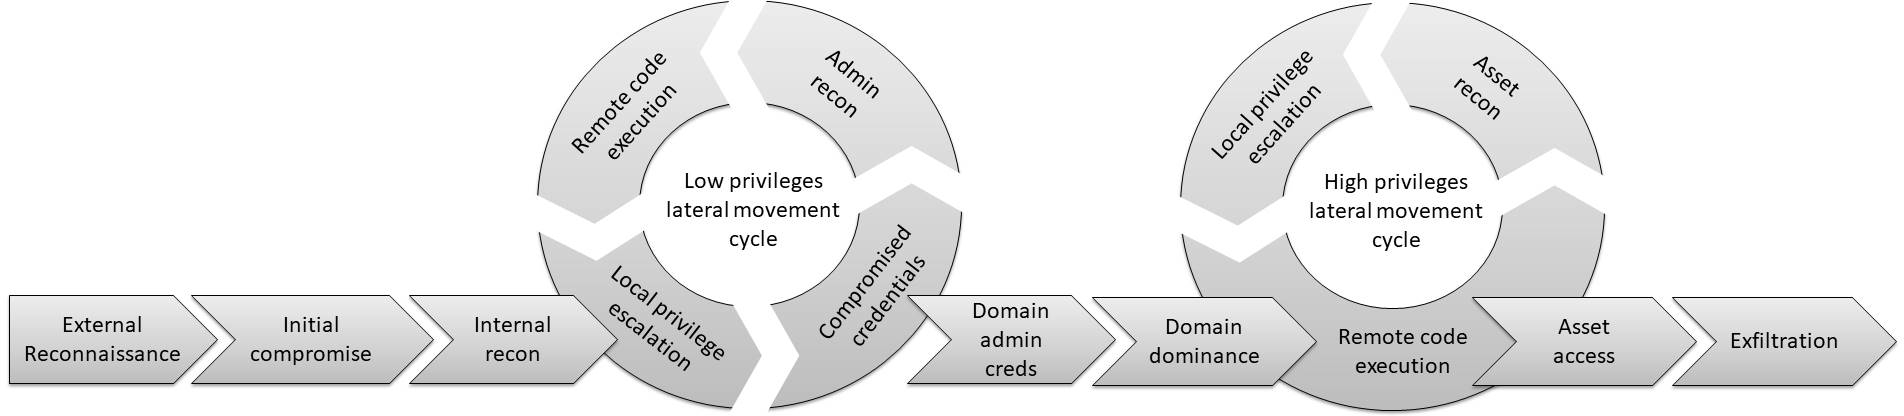
\includegraphics[width=1.0\textwidth]{./img/attack-kill-chain.jpg}
    \caption{Microsoft Attack Kill Chain \cite{Microsoft2018}}
    \label{fig:akchain}
\end{figure}

To address the strengths, weaknesses, and synergies of the popular cyber kill-chains, the author proposes an unified cyber attack kill-chain approach (Table \ref{tab:achain} on page \pageref{tab:achain}, column ``Cyber Attack Kill Chain''). The proposed model (Fig. \ref{fig:cakchain}) consists of the following phases: reconnaissance, initial compromise and foothold, command and control, internal reconnaissance, lateral movement, privilege escalation, persistence, asset reconnaissance, and objective completion. In this model, the reconnaissance and persistence loops are intertwined, with internal reconnaissance permitting lateral movement, privilege escalation and persistence, and allowing to conduct further reconnaissance activities on intended targets. If any applicable information or vulnerability is identified within the reconnaissance and lateral movement phases, the privilege escalation and persistence can be performed if necessary. However, not always privilege escalation and persistence are required to achieve the designated effect, therefore objective can be accomplished as soon as the intended target is located and the adequate network position and level of privileges have been obtained to perform the assigned task.

\begin{figure}[!htb]
    \centering
    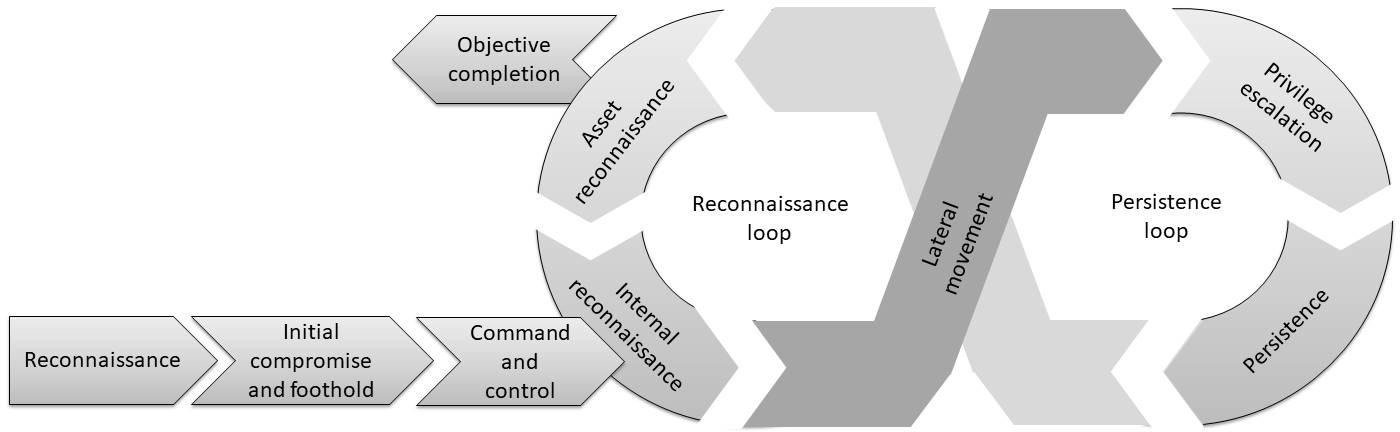
\includegraphics[width=1.0\textwidth]{./img/cyber-attack-kill-chain.jpg}
    \caption{Proposed cyber attack kill-chain model}
    \label{fig:cakchain}
\end{figure}

As stated in the chapter \ref{sec:scrtop}, such specialized cyber red team responsive operations should be capable of delivering the maximum possible effect. With this in mind, the red team needs to ensure highest success rate at every performed stage matching the cyber attack kill-chain. Such procedures would allow the applicable technique and tool proper use for accomplishing the mission objectives, maintaining the \gls{opsec}, and own asset protection.


\subsection{Chapter Conclusions}
The table \ref{tab:scrt} on page \pageref{tab:scrt} shows that the proposed methods and techniques in the research papers, are applicable to the specialized \gls{crt} responsive \gls{cno} and cover all of the aspects of such operational \gls{tttp} and demands. The majority of the proposed methods support the custom technique and tool development aimed at specific elements of the targeted system. This, with according tactics and procedures, results in a higher stealth level since these attacks are tailored to the intended objective to deliver the desired operational effects with highest impact possible. Additionally, these techniques are aimed at high stealth to provide a higher operational success rate, such as, establishing \gls{cnc} channel to circumvent the \gls{nids}. The tables \ref{tab:fuzz} and \ref{tab:tun} compare the author's developed methods against the other popular solutions. These unique and bespoke techniques are more effective when compared to relevant and commonly used ones (\ref{pub:firstPub}), grant the ease and flexibility to increase the speed of operation execution (\ref{pub:secondPub}), and allow focus of force on the most critical components of the target system (\ref{pub:thirdPub}). Based on the validated research in the publications, there are no other identified known approaches publicly available to match the level of the developed and presented techniques and tools. All of the proposed new techniques in this chapter have been implemented into the cyber red team oriented technical exercise series ``Crossed Swords'' and is described in a more detail in the chapter \ref{sec:exercises}.

A new unified cyber attack kill-chain method is introduced (Fig. \ref{fig:cakchain}) to find the synergies among the accepted kill-chain models to mitigate the gaps and emphasize their strengths.
The methods and approaches, proposed in the publications, are aimed at producing the desired effect and objective completion in the final stages of the cyber attack kill-chain. As it is identified, they cover all of the kill-chain stages either directly or can be used to support countering most of the stages, such as, allowing a local privilege escalation exploit delivery to the target system over the established covert \gls{cnc} channel.
The ultimate goal for the presented techniques is to grant the most benefit to the \gls{crt} from both the operation execution and objective accomplishment. When comparing their applicability both to specialized \gls{crt} responsive \gls{cno} execution and countering the cyber attack kill-chain, it can be assessed, that they provide a balanced approach and support to achieving the presented demands.
